\documentclass[t]{beamer}
\usepackage{media9}
\usepackage{graphicx}
\usepackage{siunitx}
\sisetup{load-configurations = abbreviations}

\mode<presentation> {
  \usetheme{boxes}
  \usecolortheme{rose}
  \setbeamertemplate{navigation symbols}{} % To remove the navigation symbols from the bottom of all slides uncomment this line
}

%\usepackage{pgfpages}
%\pgfpagesuselayout{2 on 1}[a4paper,border shrink=5mm]

\usefonttheme[onlymath]{serif}
\usepackage{fontspec} 
\defaultfontfeatures{Mapping=tex-text} 
\setsansfont[Ligatures={Common}]{Futura}
\setmonofont[Scale=0.8]{Monaco} 

\usepackage{graphicx} % Allows including images
\usepackage{booktabs} % Allows the use of \toprule, \midrule and \bottomrule in tables

%----------------------------------------------------------------------------------------
% New Commands
%----------------------------------------------------------------------------------------

\newcommand*{\movie}[1]{\includemedia[width=0.6\linewidth,height=0.3375\linewidth, activate=pageopen]{}{#1}}
\newcommand{\img}[1]{\includegraphics[width=1\linewidth]{images/#1}}
\newcommand{\imgs}[1]{\includegraphics[width=.75\linewidth]{images/#1}}
\newcommand{\imgss}[1]{\includegraphics[width=.5\linewidth]{images/#1}}
\newcommand{\bi}{\begin{itemize}}
\newcommand{\ei}{\end{itemize}}

%----------------------------------------------------------------------------------------
%	TITLE PAGE
%----------------------------------------------------------------------------------------
\title[Topic 2]{Grade 8 - Light and Optics} % The short title appears at the bottom of every slide, the full title is only on the title page
\subtitle{Topic 2: Reflections}
\author{Dr. Pineda} 
\institute[] {\href{http://www.drpineda.ca}{www.drpineda.ca}}
\date{} % Date, can be changed to a custom date

% Customize the footline
%\setbeamertemplate{footline}{goo \insertframenumber \insertsubtitle \inserttitle}

\setbeamertemplate{footline}{
   \begin{beamercolorbox}[ht=4ex,leftskip=.2cm,rightskip=.2cm]{author in head/foot}
    \usebeamercolor{UniBlue}
    \hrule
    \vspace{0.1cm}
    \inserttitle \ - \insertsubtitle \hfill \insertframenumber/\inserttotalframenumber
   \end{beamercolorbox}
   \vspace*{0.1cm}
} 

%----------------------------------------------------------------------------------------
%	BEGIN DOCUMENT
%----------------------------------------------------------------------------------------
\begin{document}

{
\setbeamertemplate{footline}{} % no page number here
\frame{\titlepage}
}

%----------------------------------------------------------------------------------------
%	PRESENTATION SLIDES
%----------------------------------------------------------------------------------------

%----------------------------------------------------------------------------------------
%	Reflection
%----------------------------------------------------------------------------------------
\begin{frame}{Reflection}
Process in which light strikes a surface and bounces back off that surface. 
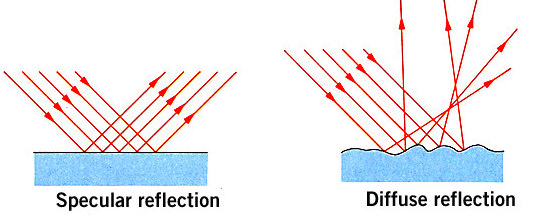
\includegraphics[width=1\linewidth]{images/specularreflection.jpg}
\end{frame}

%----------------------------------------------------------------------------------------
%	Specular vs. Diffuse Reflection
%----------------------------------------------------------------------------------------
\begin{frame}{Specular vs. Diffuse Reflection}

\begin{description}
\item[Specular reflection:]  Mirror-like reflection of light from a surface, in which light from a single incoming direction (a ray) is reflected into a single outgoing direction. A smooth surface will have all light reflect together and form a clear image

\item[Diffuse reflection:]  Reflection of light from a surface such that an incident ray is reflected at many angles rather than at just one angle as in the case of specular reflection. A rough surface will scatter light and will not form a clear image
\end{description}
\end{frame}

%----------------------------------------------------------------------------------------
%	Scientific Law
%----------------------------------------------------------------------------------------
\begin{frame}{Scientific Law}
\bi
\item A scientific law is a statement of a pattern that has been observed and tested again and again with the same results each time. \item Scientific laws \underline{do not explain why} we see a pattern.
\ei
\img{law-of-gravity-enforced.jpg}
\end{frame}

%----------------------------------------------------------------------------------------
%	Law of Reflection
%----------------------------------------------------------------------------------------
\begin{frame}{Law of Reflection}
\bi
\item Angle of incidence equals the angle of reflection
\item The incident and reflected rays and the normal are all on the same plane
\ei
\img{law_of_reflection.png}
\end{frame}

%----------------------------------------------------------------------------------------
%	How do we see reflections?
%----------------------------------------------------------------------------------------
\begin{frame}{How do we see reflections?}
\imgs{mirror.jpg}
\end{frame}

%----------------------------------------------------------------------------------------
%	How do we see reflections?
%----------------------------------------------------------------------------------------
\begin{frame}{How do we see reflections?}
The distance between object and plane (mirror surface) is same as distance between plane and virtual image.
\end{frame}

%----------------------------------------------------------------------------------------
%	Concave vs. Convex Surfaces
%----------------------------------------------------------------------------------------
\begin{frame}{Concave vs. Convex Surfaces}
\begin{description}
\item[Concave:] \only<beamer>{The surface "caves" inwards}
\item[Convex:] \only<beamer>{The surface pushes or bulges outwards}
\end{description}
\imgs{spoon.jpg}
\end{frame}

%----------------------------------------------------------------------------------------
%	The Many Uses of Reflections
%----------------------------------------------------------------------------------------
\begin{frame}{The Many Uses of Reflections}
\bi
\item Reflectors on cars and bikes, safety clothes
\item Sideview mirrors on cars are convex
\item Security mirrors in stores are convex
\item Regular mirrors
\item Funhouses to make weird body images
\item To see around corners
\item Fiber Optics
\ei
\end{frame}

%----------------------------------------------------------------------------------------
%	The Many Uses of Reflections: Fiber Optics
%----------------------------------------------------------------------------------------
\begin{frame}{The Many Uses of Reflections: Fiber Optics}
\img{fiber-optic-transmission.jpg}
\end{frame}

%----------------------------------------------------------------------------------------
%	The Many Uses of Reflections: Fiber Optics
%----------------------------------------------------------------------------------------
\begin{frame}{The Many Uses of Reflections: Fiber Optics}
Fiber optics work on the principle of total internal reflection.  Light energy carrying a signal does not escape.  It just keeps on being reflected continuously until the end. And since light travels at \SI[per-mode = symbol]{300000}{\km\per\s}, it reaches its destination almost instantaneously here on Earth.  That's why they are used for fast telecommunication (telephone signals, computer signals)
\img{optical-fiber-cable.jpg}
\end{frame}

%----------------------------------------------------------------------------------------
%	Sharks like fiber optic cables too
%----------------------------------------------------------------------------------------
\begin{frame}{\href{http://drpineda.ca/classroom/notes/Science8/LightAndOptics/media/Fiber-optic-shark-bite.html}{Sharks like fiber optic cables too (video)}}
Sharks and other fish are attracted to the cables, possibly due to the electromagnetic signals emitted by the cables. Although the cables already have protective materials designed to shelter them from the various dangers of the environment, they are easily damaged. After an underwater camera in 2010 recorded a shark taking bite out of a fiber optic trans-Pacific cable belonging to Google, the company is now reinforcing its underwater fibre-optic cables with an extra layer of protective material in order to protect its 100,000 miles of cables from sharks.
\end{frame}


%----------------------------------------------------------------------------------------
%	The Many Uses of Reflections: Archimedes' Burning Mirrors
%----------------------------------------------------------------------------------------
\begin{frame}
\frametitle{The Many Uses of Reflections: \href{http://drpineda.ca/classroom/notes/Science8/LightAndOptics/media/Archimedes-burning-mirrors.html}{Archimedes' Burning Mirrors (Video)}}
Draw a labelled sketch and write an explanation explaining how Archimedes' Burning Mirrors was supposed to work. 
\end{frame}

%----------------------------------------------------------------------------------------
%	The Many Uses of Reflections: Solar Thermal Power
%----------------------------------------------------------------------------------------
\begin{frame}
\frametitle{The Many Uses of Reflections: \href{http://drpineda.ca/classroom/notes/Science8/LightAndOptics/media/Solar-thermal-power.html}{Solar Thermal Power (Video)}}
Make a labelled sketch and write an explanation explaining how a solar thermal power plant works.
\end{frame}

\end{document}